% !TEX root = ../final_report.tex
\appendix
\section*{Appendices}
\addcontentsline{toc}{section}{Appendices}
\renewcommand{\thesubsection}{\Alph{subsection}}

\subsection{Application Repository}
\label{appendix:code}
\rule{\textwidth}{0.4pt}

\subsubsection{Location}
The Git repository for this project is available here: \newline \url{https://github.com/StephenCoady/lifecycle-management-for-docker}.

\subsubsection{Contributing}
Since this project is open source anybody is welcome to contribute. To do so:
\begin{enumerate}
	\item Clone the repository
	\item Make a branch
	\item Make the changes you want
	\item Submit a pull request on your code
\end{enumerate}
Once the pull request has then been reviewed it will be merged into the main code base.
\subsubsection{Raising an issue}
If you find a bug, please raise an issue on Github and it will then be resolved as soon as possible. 

\subsubsection{Running the application}
If you wish to run the application please first clone the repository and then run `node index.js' from within the directory.

Alternatively, you can use Docker. To do this please follow the instructions found in the README.md file in the repository.
\clearpage

\subsection{Travis Repository} 
\label{appendix:travis}
\rule{\textwidth}{0.4pt}
\subsubsection{Location}
The repository can be found at:  \url{https://travis-ci.org/StephenCoady/lifecycle-management-for-docker}

\subsubsection{Build Statistics}
We can see some statistics for the builds of this project below in Figure \ref{fig:build-stats}.

\begin{figure}[!ht]
\centering
\includegraphics*[width=0.4\textwidth]{images/build-stats}
\caption{\em Project Build Statistics}
\label{fig:build-stats}
\end{figure}

We can also see the builds per day and time taken per day to complete a build below in Figures \ref{fig:builds-per-day} and \ref{fig:build-time}.

\begin{figure}[!ht]
\centering
\begin{minipage}{.5\textwidth}
  \centering
  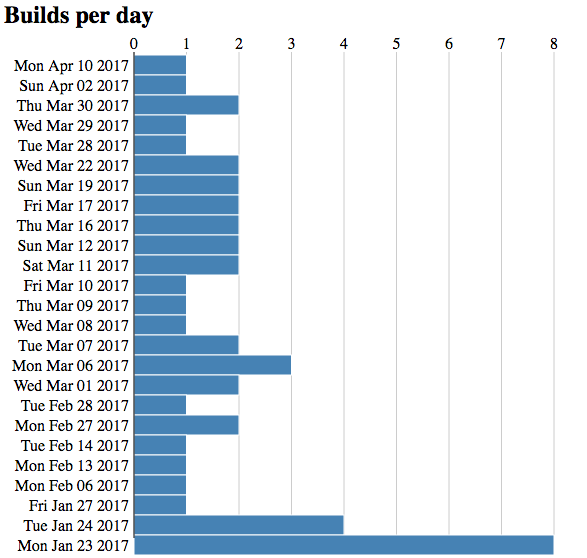
\includegraphics[width=\linewidth]{images/builds-per-day}
	\caption{\em Project Builds per Day}
	\label{fig:builds-per-day}
\end{minipage}%
\begin{minipage}{.5\textwidth}
  \centering
  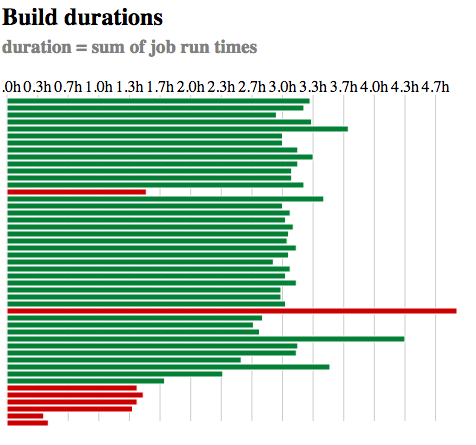
\includegraphics[width=\linewidth]{images/build-time}
	\caption{\em Project Average Build Time}
	\label{fig:build-time}
\end{minipage}
\end{figure}
\clearpage

\subsection{SonarQube Repository} 
\label{appendix:sonarqube}
\rule{\textwidth}{0.4pt}
\subsubsection{Location}
The SonarQube quality gate for this application can be found at:
\url{https://sonarqube.com/dashboard?id=lifecycle-management-for-docker}

\subsubsection{Quality Statistics}

We can see the overall SonarQube analysis statistics below in Figure \ref{fig:sonar-summary}.
\begin{figure}[!ht]
\centering
\includegraphics*[width=0.4\textwidth]{images/sonar-summary}
\caption{\em SonarQube Statistics}
\label{fig:sonar-summary}
\end{figure}

\subsubsection{Code Coverage}
In Figure \ref{fig:code_coverage} below we can see that the code coverage for this project was consistently maintained at 90\%.

\begin{figure}[!ht]
\centering
\includegraphics*[width=\textwidth]{images/code_coverage}
\caption{\em Code Coverage}
\label{fig:code_coverage} 
\end{figure}

Technical debt was also focused on and as a result was maintained at an average 30 minutes for the duration of the project. This can be seen in Figure \ref{fig:technical-debt}.
\clearpage
\begin{figure}[!ht]
\centering
\includegraphics*[width=\textwidth]{images/technical-debt}
\caption{\em Technical Debt}
\label{fig:technical-debt} 
\end{figure}

The number of \glspl{code smell} was also maintained as low as possible, with the number averaging at 10. This can be seen below in Figure \ref{fig:code_smell}.

\begin{figure}[!ht]
\centering
\includegraphics*[width=\textwidth]{images/code_smell}
\caption{\em Code Smell}
\label{fig:code_smell} 
\end{figure}

\clearpage

\subsection{DockerHub Repository} 
\label{appendix:dockerhub}
\rule{\textwidth}{0.4pt}

\subsubsection{Location}
The repository for the Docker image of this project can be found at: \url{https://hub.docker.com/r/scoady2/lifecycle-management-for-docker/}

\subsubsection{Running The Container}
To run the container Docker must first be installed on the desired system. Once Docker is installed the command: 
\begin{figure}[!ht]
\begin{lstlisting}
docker run -d -p 3000:3000 -v /var/run/docker.sock:/var/run/docker.sock scoady2/lifecycle-management-for-docker 
\end{lstlisting}
\end{figure}

will start the container.

\subsection{Staging Server} 
\label{appendix:staging}
\rule{\textwidth}{0.4pt}

This application is staged on a public instance which can be accessed at: \newline
application: \url{http://87.44.18.55:3000/} \newline
documentation: \url{http://87.44.18.55:3000/docs}

To use the application one must first log in, this can be done using the username and password provided below.\newline
username: admin \newline
password: admin

\subsection{Report Source Code} 
\label{appendix:reports}
\rule{\textwidth}{0.4pt}

All \LaTeX\  files for this paper are available here: \url{https://github.com/StephenCoady/college-papers}

\clearpage
\subsection{Formal System Models}
\label{appendix:models}
\rule{\textwidth}{0.4pt}

\subsubsection{Class Diagram}
\begin{figure}[!ht]
\centering
\makebox[\textwidth]{\includegraphics*[width=0.9\paperwidth]{images/models/docker_class_diagram}}
\caption{\em Class Diagram}
\label{fig:class-diagram}
\end{figure}

We can see the class diagram for this system in Figure \ref{fig:class-diagram}. Each class is explained below in list form.

\begin{itemize}
	\item Container - the container on the system, state is either running or not running. It is run from an existing image on the system.
	\item Image - the template from which a container is created. May be local or remote.
	\item Dockerfile - the template from which an image is built. Each line in the Dockerfile leads to a unique Docker image.
	\item Repository - a remote location where images can be pushed. For an example of a Docker repository please see Appendix \ref{appendix:dockerhub}.
	\item Registry - a remote location which houses one or more repositories.
\end{itemize}

\subsubsection{Sequence Diagrams}

An example of how the sequence diagram shown in Figures \ref{fig:sequence-diagram} and \ref{fig:user-sequence-diagram} should be read is:
\begin{legal}
	\item The web server calls the list container API endpoint
	\begin{legal} 
		\item the endpoint passes the container ID to the Docker API 
	\begin{legal} 
		\item if the container exists the docker daemon acknowledges this 
		\item the container is then returned to the Docker API 
	\end{legal}
	\item the Docker API returns an OK status message and also the container information 
	\item the API returns the container information in JSON form 
	\end{legal}
\end{legal}

\begin{figure}[!ht]
\centering
\makebox[\textwidth]{\includegraphics*[width=0.9\paperwidth]{images/models/docker_system}}
\caption{\em Sequence Diagram}
\label{fig:sequence-diagram}
\end{figure}
\clearpage

\begin{figure}[!ht]
\centering
\makebox[\textwidth]{\includegraphics*[width=0.8\paperwidth]{images/models/user_system}}
\caption{\em User System Sequence Diagram}
\label{fig:user-sequence-diagram}
\end{figure}

\begin{figure}[!ht]
\centering
\makebox[\textwidth]{\includegraphics*[width=0.9\paperwidth]{images/models/use_case}}
\caption{\em Use Case Diagram}
\end{figure}

\textbf{Authenticate User Remotely} - if the user wishes to push or pull to/from a remote repository then they must login\newline
\textbf{Push Image} - the act of pushing an image from a local machine to a remote one\newline
\textbf{Pull Image} - finding an image not currently on the system and making it available by `pulling' it from a repository\newline
\textbf{List} - getting a list of all containers/images on a host\newline
\textbf{Delete} - remove a container/image from a host\newline
\textbf{Start} - start a container from an image on a host\newline
\textbf{Authenticate Locally} - if a user wishes to perform any action on the Docker engine they must be authenticated. This is always true unless the Docker remote API has been restricted\newline


\clearpage
\subsection{Wireframes}
\label{appendix:wireframes}
This is the landing page when the application is first visited. It will show a few high level details about the host.

\begin{figure}[!ht]
\centering
\includegraphics*[width=0.9\textwidth]{wireframes/dashboard}
\caption{\em Dashboard Mockup}
\end{figure}
This is the container control view. It shows the main view which can be used to perform most actions on containers.

\begin{figure}[!ht]
\centering
\includegraphics*[width=0.9\textwidth]{wireframes/container}
\caption{\em Container Mockup}
\end{figure}
This is the image control view. It shows the main view which can be used to perform most actions on images.

\begin{figure}[!ht]
\centering
\includegraphics*[width=0.9\textwidth]{wireframes/images}
\caption{\em Images Mockup}
\end{figure}
The individual view for an image. It will give a high level overview of that image.

\begin{figure}[!ht]
\centering
\includegraphics*[width=0.9\textwidth]{wireframes/image}
\caption{\em Image Mockup}
\end{figure}
\clearpage
This is the network control view. It shows the main view which can be used to perform most actions on networks.

\begin{figure}[!ht]
\centering
\includegraphics*[width=0.9\textwidth]{wireframes/networks}
\caption{\em Networks Mockup}
\end{figure}
The individual view for a network. It will give a high level overview of that network.

\begin{figure}[!ht]
\centering
\includegraphics*[width=0.9\textwidth]{wireframes/network}
\caption{\em Network Mockup}
\end{figure}

\newpage
This page will give all relevant information about the Docker installation.
\begin{figure}[!ht]
\centering
\includegraphics*[width=0.9\textwidth]{wireframes/docker}
\caption{\em Docker Mockup}
\end{figure}
This page shows the host information page. Any relevant information which shows details of the host Docker is installed on will be displayed here.

\begin{figure}[!ht]
\centering
\includegraphics*[width=0.9\textwidth]{wireframes/host}
\caption{\em Host Mockup}
\end{figure}
